%%%% CAPÍTULO 4 - RESULTADOS E DISCUSSÃO

\chapter{Experimentação}\label{cap:experimentos}

Esta seção apresenta a execução dos experimentos previstos na metodologia,
descrevendo a preparação do objeto experimental, a extração das
\textit{bufferViews} e o comportamento da camada física durante o processo de
versionamento. Essas etapas permitem compreender como o método é aplicado antes da
apresentação dos resultados quantitativos.

\section{Preparação do objeto experimental}

O objeto experimental utilizado consiste no modelo tridimensional
\texttt{ABeautifulGame.glb}, disponibilizado pelo Khronos Group
\cite{KhronosSamples2026}. O modelo apresenta tamanho de 42,9 MB e é composto por
108 \textit{bufferViews}, das quais 75 armazenam dados de geometria e 33
correspondem a índices e demais informações estruturais.

Uma limitação do modelo consiste na ausência de animações. Em razão dessa
característica, os cenários experimentais concentram-se exclusivamente em
modificações aplicadas aos dados de geometria, permitindo avaliar o comportamento do
mecanismo de versionamento diante de alterações estruturais no modelo
tridimensional.

\section{Extração das bufferViews}

No modelo \texttt{ABeautifulGame}, utilizado nos experimentos, esse processo
resultou em 108 \textit{bufferViews} extraídas de um total de 42,9 megabytes,
distribuídas em segmentos com tamanhos variando de 9.376 \textit{bytes} a 1.843.200
\textit{bytes}, correspondendo a atributos de vértices, normais, coordenadas de
textura e índices de face de 15 malhas diferentes.

\section{Funcionamento da camada física}

A Figura~\ref{fig:camada-fisica-inicial} apresenta o estado inicial da camada
física, correspondente ao primeiro \textit{snapshot}, composto pela raiz inicial,
pelos nós internos A e B e pelos nós folha contendo as \textit{bufferViews}
originais.

\begin{figure}[htb]
  \centering
  \caption{\label{fig:camada-fisica-inicial}Camada física de uma versão inalterada}
  \fbox{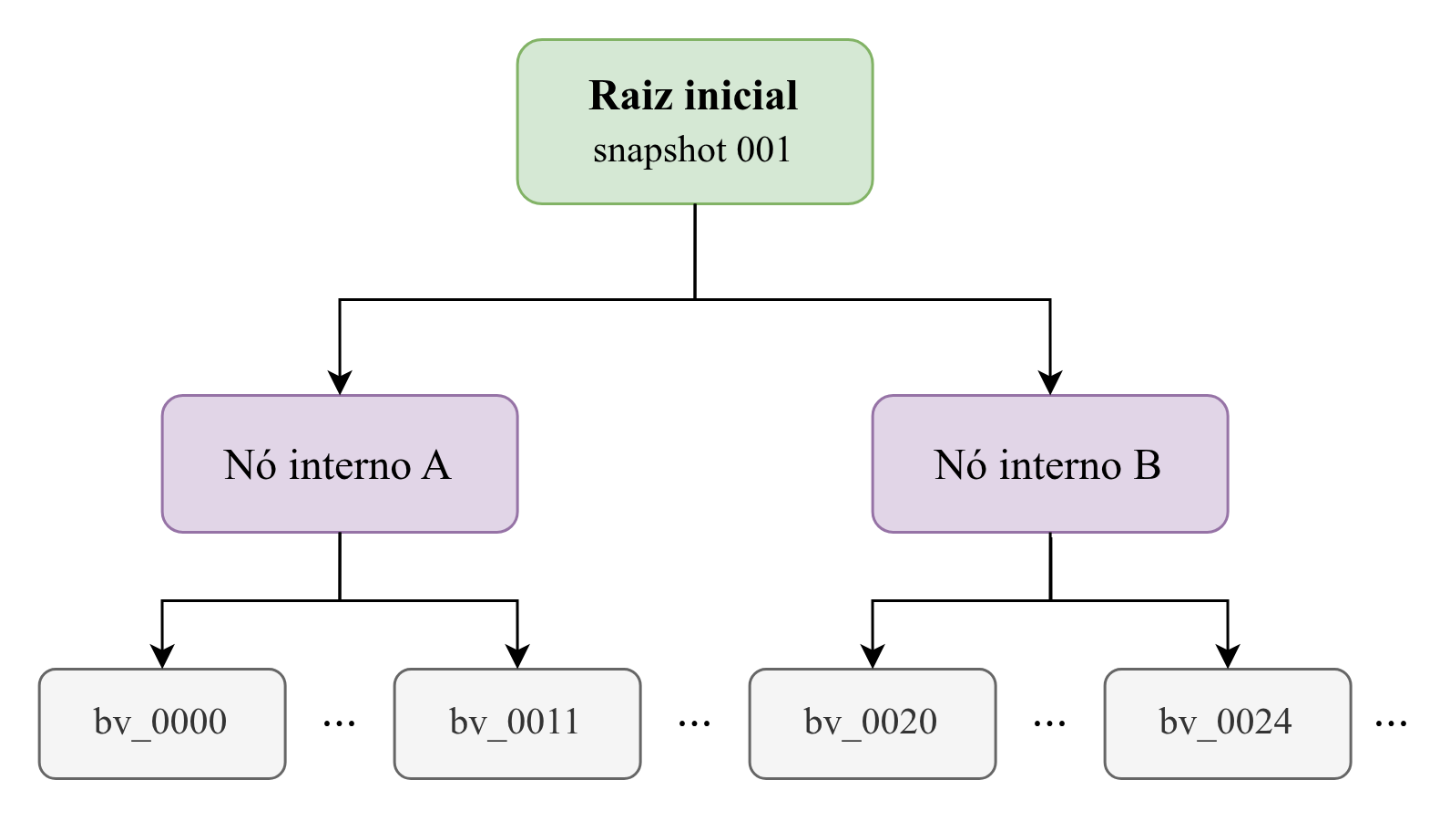
\includegraphics[width=0.8\textwidth]{figuras/camada-fisica-inalterada.png}}
  \fonte{Autoria própria (2026)}
\end{figure}

A Figura~\ref{fig:camada-fisica-alterada} ilustra o estado da camada física após o
registro de uma nova versão contendo uma modificação na \textit{bufferView}
\texttt{bv\_0011}. O mecanismo \gls{cow} do \gls{btrfs} aloca um novo nó folha para
armazenar o conteúdo atualizado, preservando o bloco original. Como a modificação
afeta apenas um ramo da árvore, o nó interno correspondente também recebe uma nova
cópia, propagando essa atualização até a raiz da árvore.

\begin{figure}[htb]
  \centering
  \caption{\label{fig:camada-fisica-alterada}Camada física de uma versão com alterações}
  \fbox{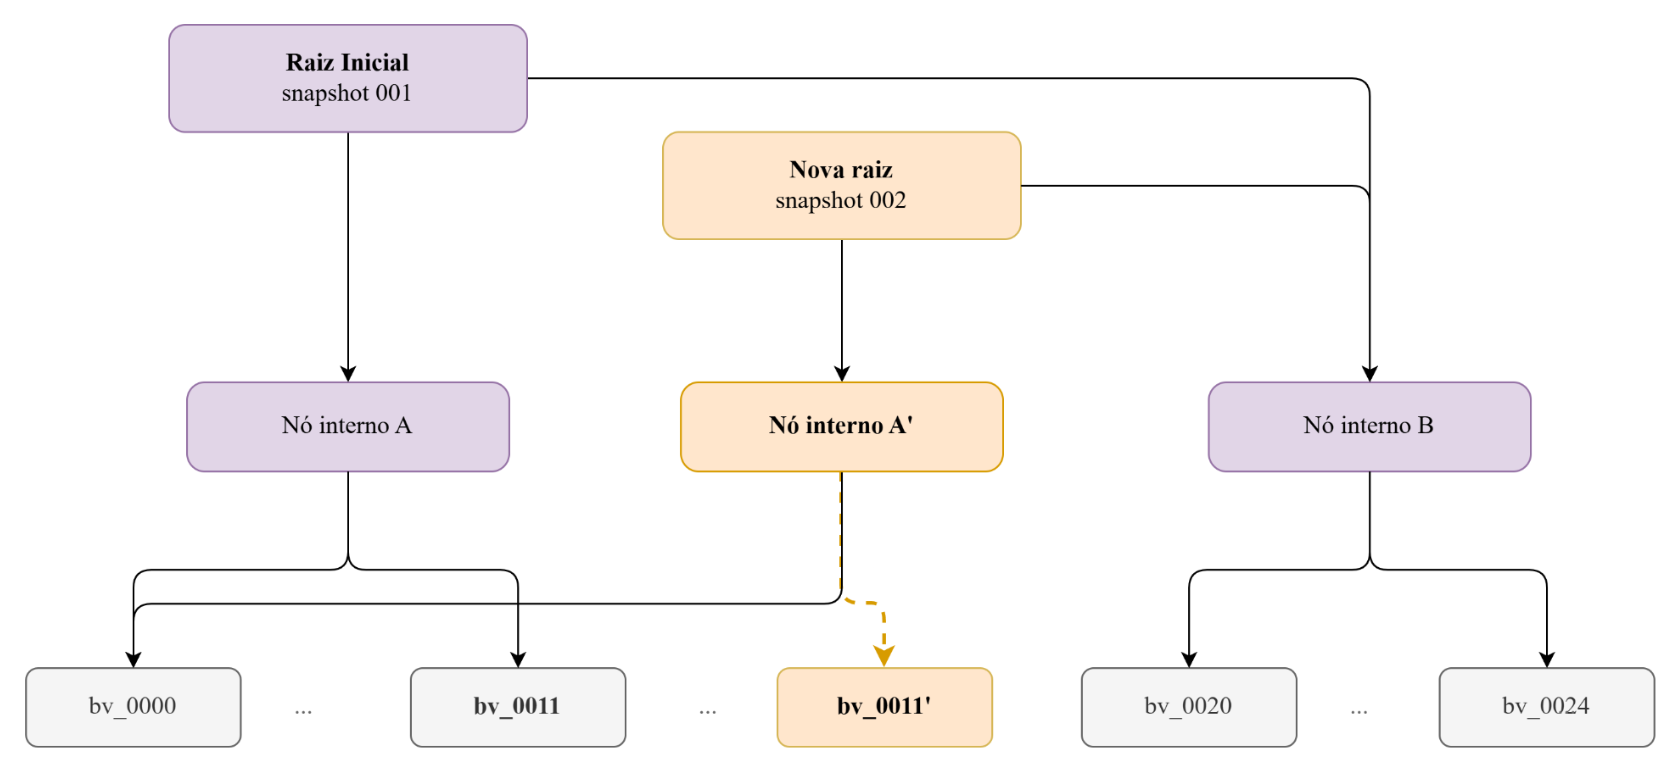
\includegraphics[width=0.8\textwidth]{figuras/camada-fisica-alterada.png}}
  \fonte{Autoria própria (2026)}
\end{figure}

Os demais ramos permanecem inalterados e continuam sendo compartilhados entre os
dois \textit{snapshots}, sem duplicação física dos dados. Dessa forma, apenas os
blocos efetivamente modificados e os metadados necessários para manter a
consistência da árvore ocupam espaço adicional no armazenamento.

\subsection{Execução dos experimentos}

Os resultados apresentados a seguir foram coletados após executar todo o ciclo
experimental nas duas máquinas virtuais, cobrindo os oito cenários de teste da
Tabela~\ref{tab:cenarios}. A primeira versão é a base, onde o modelo
\texttt{ABeautifulGame} é salvo sem nenhuma mudança. As versões seguintes mostram
modificações progressivas aplicadas apenas aos dados de geometria, variando de 2\% a
90\% das \textit{bufferViews}.

No método de referência, usando o \gls{gitlfs}, observou-se que aproximadamente 42,9
MB foram adicionados ao armazenamento no \gls{gitlfs} a cada nova versão, sem
importar o quanto a modificação era grande. Ao final das oito versões, o
armazenamento no \gls{gitlfs} acumulou 343,9 MB de dados. Isso significa que 8
cópias completas do arquivo foram guardadas. Esse comportamento já era esperado pela
forma como o \gls{gitlfs} funciona: como ele trata o arquivo \gls{glb} como um bloco
único, qualquer mudança no seu conteúdo gera um identificador único diferente. Isso
força o sistema a guardar um novo arquivo completo, mesmo que a alteração tenha sido
pequena.

Já no método proposto, o comportamento foi diferente. A versão 1, que é a primeira
vez em que o modelo é salvo, precisou gravar todas as 108 \textit{bufferViews},
totalizando 42,9 MB, pois não havia uma versão anterior para comparar. A partir da
versão 2, o sistema percebeu que 75 \textit{bufferViews} tinham sido modificadas e
33 continuavam iguais. Isso resultou na gravação de 24,0 MB por versão e uma
economia de 44,08\% em relação ao tamanho total do arquivo. Esse padrão se manteve
em todas as versões seguintes. Isso acontece porque a detecção de diferenças
funciona comparando os identificadores únicos das \textit{bufferViews} entre as
versões e qualquer mudança nos \textit{bytes} de uma \textit{bufferView}, por menor
que seja, muda seu identificador e a marca como modificada. As \textit{bufferViews}
que não foram alteradas são ignoradas no processo de escrita. Como os oito cenários
de teste sempre modificam o mesmo grupo de 75 \textit{bufferViews} de geometria,
variando apenas a intensidade das mudanças numéricas, o número de segmentos gravados
permaneceu o mesmo entre as versões. A Tabela~\ref{tab:resultados-exp1} resume os
resultados coletados em ambas as instâncias durante o experimento.

\begin{table}[htb]
  \centering
  \caption{\label{tab:resultados-exp1}Comparativo de custos de armazenamento por versão}
  \begin{tabular}{ccccc}
    \toprule
    \textbf{Versão} & \textbf{Modificação (\%)} & \textbf{Btrfs gravado (MB)} &
    \textbf{Btrfs economia (\%)} & \textbf{Git LFS gravado (MB)} \\
    \midrule
    1 & 0  & 42 & 0,00  & 42 \\
    2 & 2  & 24 & 44,08 & 42 \\
    3 & 5  & 24 & 44,08 & 42 \\
    4 & 10 & 24 & 44,08 & 42 \\
    5 & 20 & 24 & 44,08 & 42 \\
    6 & 30 & 24 & 44,08 & 42 \\
    7 & 50 & 24 & 44,08 & 42 \\
    8 & 70 & 24 & 44,08 & 42 \\
    \midrule
    Total & --- & 210 & --- & 336 \\
    \bottomrule
  \end{tabular}
  \fonte{Autoria própria (2026)}
\end{table}

Ao final das oito versões, o armazenamento acumulado foi de cerca de 211 MB no
método proposto, contra 344 MB no \gls{gitlfs}. Isso representa uma redução de
38,6\% no uso total de espaço em disco. É importante notar que a economia do método
proposto pode ser ainda maior em situações onde as mudanças atingem um número menor
de \textit{bufferViews}. Isso acontece porque a precisão da detecção de mudanças
depende da estrutura interna do arquivo, e não da quantidade total de dados que foi
alterada.

Sobre o segundo método experimental proposto se analisa os seguintes resultados. No
método de referência, utilizando o \gls{gitlfs}, observou-se um comportamento
consistente de armazenamento. A cada nova versão, aproximadamente 42,9 MB foram
adicionados ao repositório, independentemente da quantidade de \textit{bufferViews}
modificadas. Ao final das oito versões, o armazenamento total acumulado no
\gls{gitlfs} atingiu cerca de 343,9 MB. A Figura~\ref{fig:modelo-modificado} ilustra
visualmente a diferença entre o modelo original e o modelo na versão 8, onde todas
as \textit{bufferViews} de atributos foram modificadas, resultando em extrusões nos
vértices, que, embora sutis, foram suficientes para acionar o mecanismo de
versionamento.

\begin{figure}[htb]
  \centering
  \caption{\label{fig:modelo-modificado}O modelo modificado}
  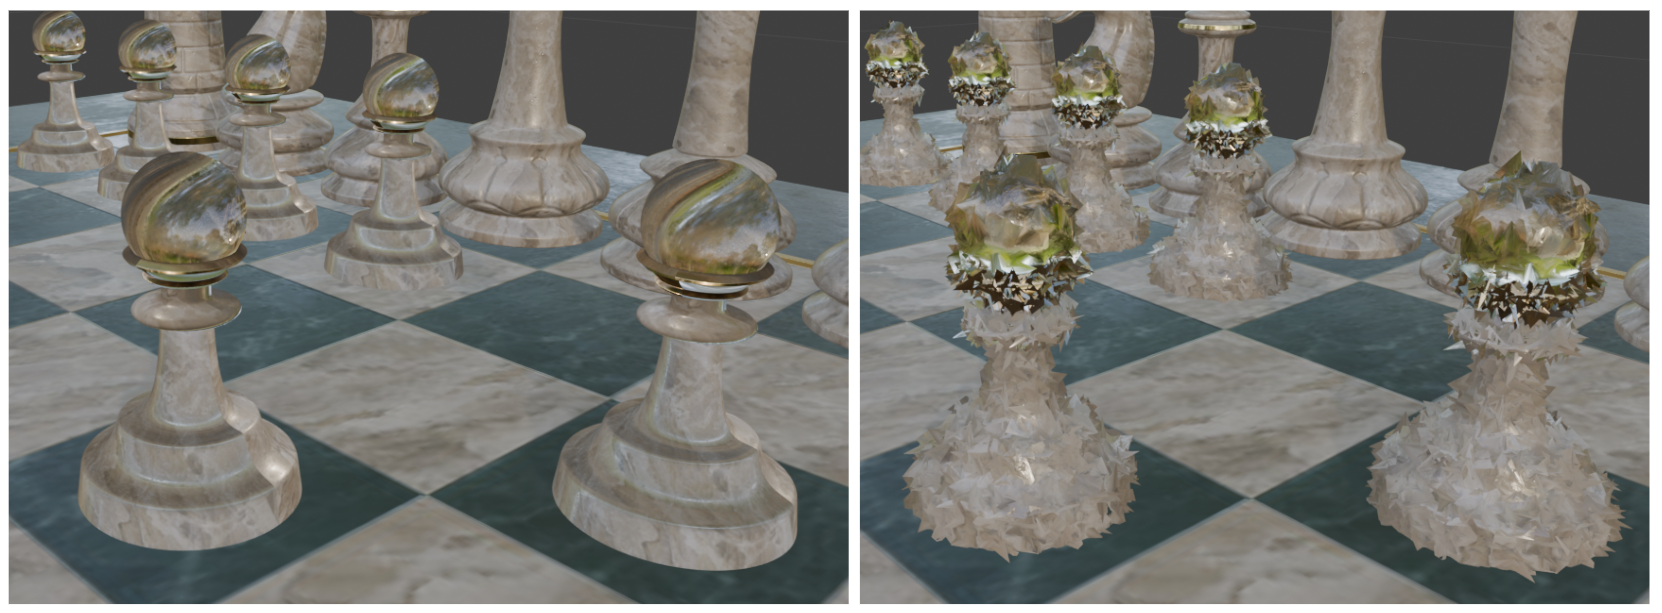
\includegraphics[width=0.8\textwidth]{figuras/modelo-modificado.png}
  \fonte{Autoria própria (2026)}
\end{figure}

Em contraste, o método proposto, baseado no \gls{btrfs}, demonstrou uma eficiência
de armazenamento significativamente superior. A versão inicial registrou 42,9 MB,
pois todas as 108 \textit{bufferViews} foram consideradas novas. A partir da segunda
versão, o sistema identificou as \textit{bufferViews} modificadas e gravou apenas os
dados correspondentes a essas alterações. Por exemplo, na segunda versão, com apenas
uma \textit{bufferView} modificada, foram gravados apenas 0,75 MB, resultando em uma
economia de 98,25\% em relação ao tamanho total do arquivo. Essa economia diminuiu
progressivamente à medida que mais \textit{bufferViews} foram modificadas, atingindo
9,31\% na oitava versão, onde 93 \textit{bufferViews} foram alteradas, com 38,9 MB
gravados. Este comportamento reflete a capacidade do \gls{btrfs} de armazenar
diferencialmente apenas os blocos de dados que sofreram alterações, compartilhando
os blocos inalterados entre as versões por meio de \textit{snapshots} \gls{cow}. Ao
final das oito versões, o armazenamento acumulado pelo método proposto foi de 211
MB, representando uma redução de 38,6\% no uso total de espaço em disco em
comparação com o \gls{gitlfs}. A Tabela~\ref{tab:resultados-exp2} resume os
resultados comparativos de armazenamento para ambos os métodos.

\begin{table}[htb]
  \centering
  \caption{\label{tab:resultados-exp2}Comparativo de custos de armazenamento}
  \begin{tabular}{crrr}
    \toprule
    \textbf{Versão} & \textbf{Btrfs gravado (\textit{bytes})} &
    \textbf{Btrfs economia (\%)} & \textbf{Git LFS gravado (\textit{bytes})} \\
    \midrule
    1 & 42.945.647  & 0,00  & 42.945.647 \\
    2 & 750.313     & 98,25 & 42.945.647 \\
    3 & 1.902.849   & 95,57 & 42.945.647 \\
    4 & 3.892.967   & 90,94 & 42.945.647 \\
    5 & 10.973.923  & 74,45 & 42.945.647 \\
    6 & 19.098.856  & 55,53 & 42.945.647 \\
    7 & 28.555.173  & 33,51 & 42.945.647 \\
    8 & 38.947.439  & 9,31  & 42.945.647 \\
    \midrule
    Total & 147.067.167 & --- & 343.565.176 \\
    \bottomrule
  \end{tabular}
  \fonte{Autoria própria (2026)}
\end{table}